\hypertarget{highly-overlapped-signals}{%
\chapter{Challenges of Highly Overlapped Signals}\label{cha:highly-overlapped-signals}}

In the previous chapter, I introduced signal processing fundamentals in the context of audio mixtures. In this chapter, I focus on the challenges of highly overlapped signals.

\hypertarget{separability-of-mixtures}{%
\section{Separability of Mixtures}\label{separability-of-mixtures}}

Time-frequency representations such as the short-time Fourier transform (STFT) have clear benefits such as the improved interpretability due to its ``image-like'' two-dimensional properties.
More importantly, however, such a representation allows to separate mixtures of speech and musical instruments.
The reason for this is that these mixtures may be fully overlapped in the time domain but are less overlapped in the frequency domain~\cite{rickard02, giannoulis11, rafii}.
In turn, a time-frequency representation allows applying to filter in a way that sufficiently extracts all targets from the mixture.
Furthermore, it allows for the reconstruction of the original waveform and provides a good trade-off between computational complexity and separation quality.
\par
Due to these reasons, many source separation methods focus on extracting individual sources by modeling their respective target in the time-frequency domain.
Further, it is assumed that the STFT provides a sufficient level of separability.
The actual extraction or filtering is done by synthesizing the magnitude estimate of the model and applying the originals mixture phase.
\par
In practice, the ability to extract a source from a mixture depends on the amount of overlap between sources.
Without any overlap, separation is not necessary, and a small amount of overlap can be tolerated to extract the sources still sufficiently.
However, if sources are fully overlapped in both, time and frequency, a separation in the TF domain is hardly possible.
A metric that is often used for evaluation is called \emph{separability} and was found by Rickard in~\cite{rickard02} as a useful metric for both, speech and music~\cite{giannoulis11} signals.
\par
In linear mixtures, separability is defined as \emph{a measure that indicates the percentage of time-frequency bins of a source is disjoint from those of interfering sources} and calculated through the W-disjoint orthogonality metric \(WDO\) in \cite{rickard02}.

If \(\mM \in \{0, 1\}^{m\times n}\) is an ideal binary mask~\cite{wang05} for a given target \(\mS\) and its interfering magnitude \(\mY\) of same dimensions as \(\mM\), the W-disjoint orthogonality metric \(WDO\) is defined as:

\begin{equation}
    PSR_{M} = \frac{\|\mM \otimes \mS_{k}\|^{2}}{\|\mS_{k}\|^{2}}
\end{equation}

\begin{equation}
    SIR_{M}=\frac{\|\mM \otimes \mS_{k}\|^{2}}{\|\mM \otimes \mY_{k}\|^{2}} 
\end{equation}

\begin{equation}
    WDO_{M} = PSR_{M} - \frac{PSR_{M}}{SIR_{M}}
\end{equation}

Where the \(PSR\) is the reserved-signal ratio, and \(SIR\) is the signal-to-interference ratio and \(\otimes\) being the element-wise product.
A \(WDO\) of one means the sources are entirely disjoint, hence no overlap.
A \(WDO\) zero means can be interpreted as sources being fully overlapped.
\par
The ability to separate sources is depending on the scenario and its applications.
Let us consider the following scenarios:

\begin{description}
  \item[Cocktail Party] where multiple speakers are speaking concurrently, it results in a partial overlap of speech signals in both time an frequency. 
  \item[Vocals and Accompaniment] are often active at the same time in professionally produced music.
  \item[Unison Instrument Mixtures] have a severe overlap in almost all active time-frequency bins.
\end{description}

Now, for these scenarios, the actual overlap depends on additional parameters like the number of sources, the class of source or the fundamental frequency.
For instance, the overlap in a cocktail party of two speakers is smaller than with ten concurrent speakers speaking.
Also, the overlap between male and female or brass and string instruments is smaller than with two instruments of the same class. 
And if two instrumental notes share the same fundamental frequency (playing in \emph{unison}), the sources are almost entirely overlapped.
\par
\begin{figure*}[hb]
\centering
\subcaptionbox[Speech]{Speech}%
[1\textwidth]{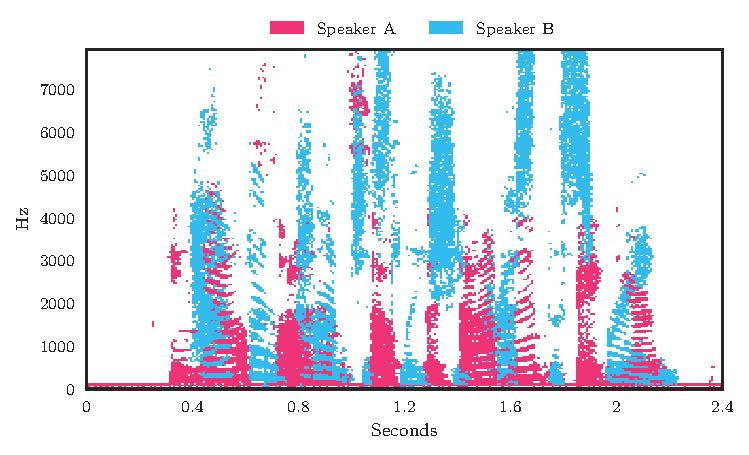
\includegraphics[width=0.8\textwidth]{Chapters/02_Fundamentals/figures/dominance_map_speakers.pdf}}%
\hspace{0.2\textwidth} % seperation
\subcaptionbox[Vocal/Accompaniment]{Vocal/Accompaniment}
[1\textwidth]{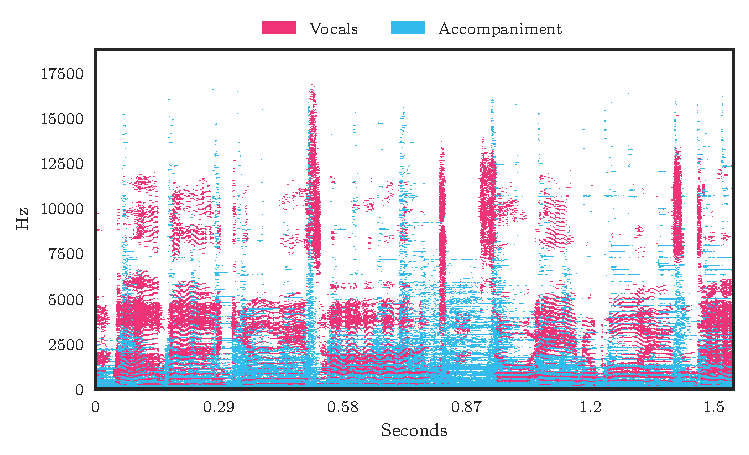
\includegraphics[width=0.8\textwidth]{Chapters/02_Fundamentals/figures/dominance_map_vocacc.pdf}}%
\hspace{0.2\textwidth} % seperation
\subcaptionbox[Speech]{Unison}
[1\textwidth]{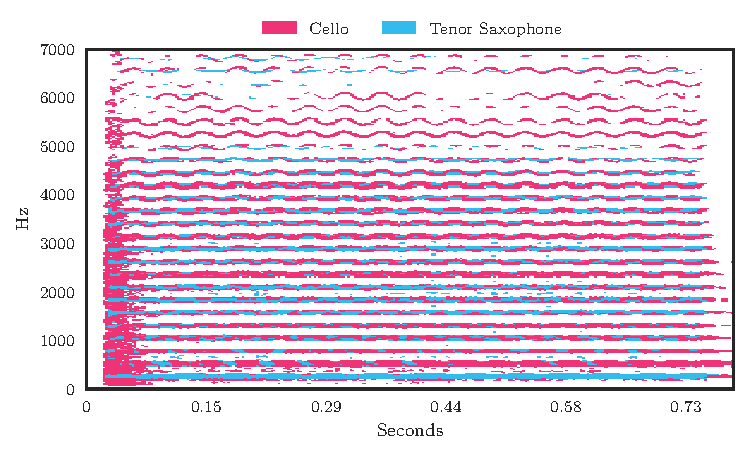
\includegraphics[width=0.8\textwidth]{Chapters/02_Fundamentals/figures/dominance_map_unison.pdf}}%
\caption{Predominant source activity, showing the predominant source for each time  frequency entry. Computed using binary masks of each source entry.}
\label{fig:dominance}
\end{figure*}

\begin{figure*}[hb]
\centering
\subcaptionbox[Speech]{Speech}%
[1\textwidth]{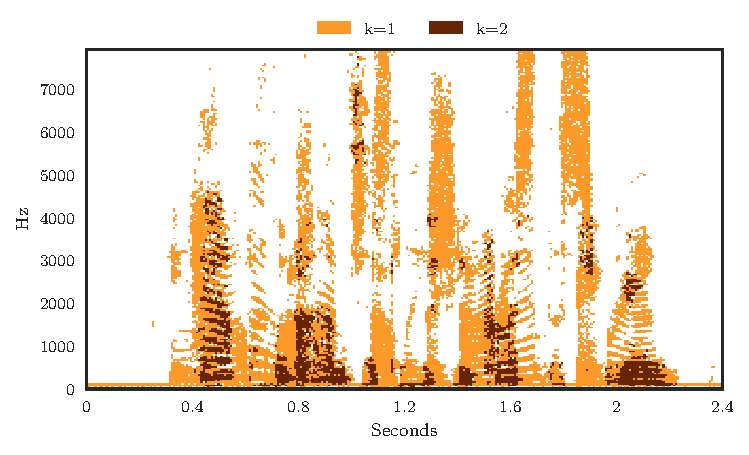
\includegraphics[width=0.8\textwidth]{Chapters/02_Fundamentals/figures/count_map_speakers.pdf}}%
\hspace{0.2\textwidth} % seperation
\subcaptionbox[Vocal/Accompaniment]{Vocal/Accompaniment}
[1\textwidth]{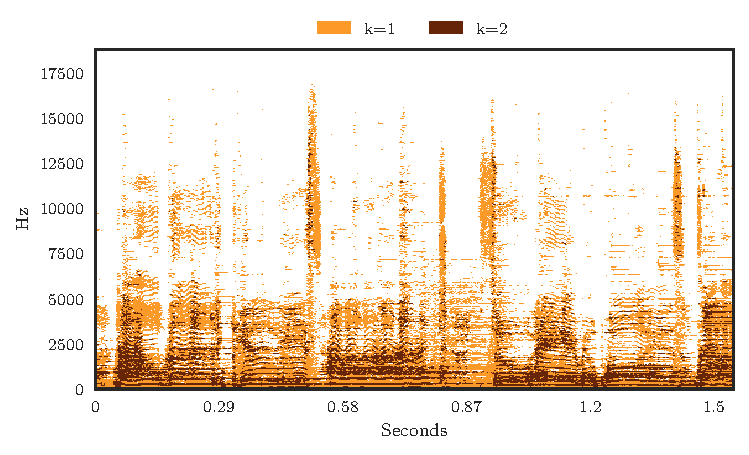
\includegraphics[width=0.8\textwidth]{Chapters/02_Fundamentals/figures/count_map_vocacc.pdf}}%
\hspace{0.2\textwidth} % seperation
\subcaptionbox[Unison]{Unison Instruments}
[1\textwidth]{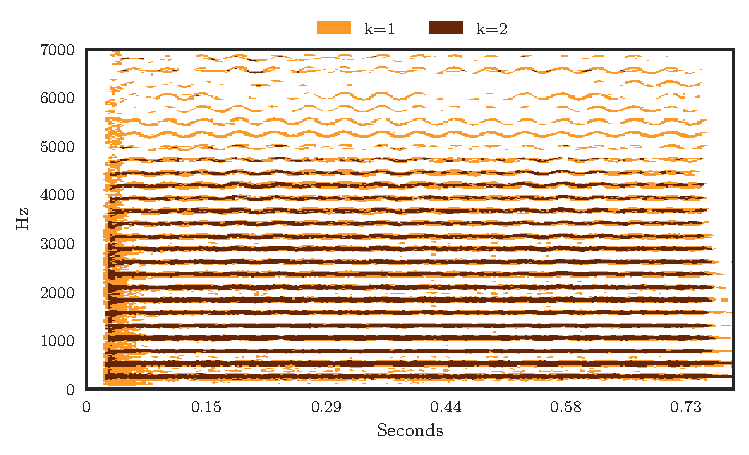
\includegraphics[width=0.8\textwidth]{Chapters/02_Fundamentals/figures/count_map_unison.pdf}}%
\caption{Source Count Activity showing the number of sources $k$ for each time frequency entry. Computed using binary masks of each source entry.}
\label{fig:count}
\end{figure*}

To illustrate this, we depict the different scenarios in two complementary figures.
Figure~\ref{fig:dominance} assigns each time-frequency entry to its predominant source.
Figure~\ref{fig:count} depicts the number of active sources (thresholded) of each TF entry.
From these figures, one can see that the overlap of a typical speech mixture is comparable to a music recording where the task is to separate vocals and accompaniment.
If we now compare this to the scenario where sources are fully overlapped as in the unison scenario, almost all TF bins are overlapped, and separation would hardly be possible.
\par
While this is an extreme scenario, it still provides a useful example where common assumptions are violated, and it would facilitate the demand to develop new methods that do not rely so much on these assumptions.
By naïvely observing the time-frequency representation in Figure~\ref{fig:count} closely, we see that the slow spectro-temporal modulations caused by the vibrato are one of the aspects where the two sources differ.
Here, the classical STFT does not provide sufficient separability and representations as in the \emph{modulation spectrogram}, presented by~\cite{greenberg96} may be preferable.
Details about this approach are discussed in Chapter~\ref{cha:unknown}.

\hypertarget{exploiting-slow-modulations}{%
\section{Exploiting Slow Modulations}\label{exploiting-slow-modulations}}

Tempo-spectral modulations occur both in speech and music signals as detailed in Section~\ref{sub:time-variant-audio-signals}.
Exploiting modulations is natural for humans: early research from Zwicker in 1952 focused on the human ability to detect amplitude modulations~\cite{zwicker52}. 
Later, it was shown by Bregman, McAdams, and Fastl in~\cite{mcadams89, bregman90, fastl90} that humans use amplitude modulations to group sources; this concept was called \emph{Common Amplitude Modulation} (CAM).
CAM exploits the fact that harmonics that share the same amplitude modulation across frequency bins are perceived \emph{integrated} as opposed to~\emph{segregated}.
Further, it was shown in~\cite{bacon89} that the ability to detect amplitude modulations can be incorporated into auditory models.
It was then found by Dau in~\cite{dau99} that humans are especially sensitive at low-frequency modulations:

\begin{quote}
``Slow modulations are associated with the perception of rhythm. Samples of running speech, for example, show distributions of modulation frequencies with peaks around 3-4 Hz, approximately corresponding to the sequence rate of syllables~\cite{plomp83}. Results from physiological studies have shown that, at least in mammals, the auditory cortex seems to be limited in its ability to follow fast temporal changes.''
\end{quote}

Dau proposed a model that mimics the ability to detect modulation patterns and pointed out applications to improve the perception for hearing-impaired listener or speech intelligibility.
\par
Previously, research has addressed a variety of tasks of processing and analysis in the context of modulations.
In the following, we give an overview of existing work focussed on analysis and separation of modulated sounds.

\subsection{Analysis}
\label{sub:modulation-analysis}}
%lets start with speech
In speech, techniques using modulation patterns improved applications such as speech  discrimination~\cite{mesgarani04} or extract spatial acoustic signatures from mixtures~\cite{sukittanon06}.
One way of analyzing amplitude modulations is to use a modulation spectrogram~\cite{greenberg97} which is a frequency-frequency representation of a time domain input signal.
In practice, the modulation spectrogram can be represented by a tensor \(\mathbf{V}_{f, b, t}\) , where \(b\) represents the modulation index, can be computed from the (magnitude) time frequency matrix \(\mathbf{X}_{f, t}\) by computing \(f\) time frequency transforms over each frequency band of \(\mathbf{X}\).
The use of modulation spectra helps to identify amplitude modulations such as the one (indirectly) caused by vibrato. 
The modulation spectrogram has already gathered much attention in speech recognition~\cite{greenberg97, kingsbury98} and classification~\cite{kinnunen08, markaki09}.
\par
Interestingly, Greenberg in~\cite{greenberg97} assumed that ``the energy in the modulation spectrum may be derived from syllabic segmentation'' and from ``the preservation of the portion of the modulation spectrum between 2 and 10 Hz''.
Following this, it was later proved that the detection of modulations improves speech intelligibility~\cite{elhilali03} or automatic speech recognition~\cite{kingsbury98}.
\par
% go to music
The analysis of amplitude modulations were also proposed for music tasks. 
Work by Scheirer in~\cite{scheirer99} proposed a method that operates by utilizing common modulation among groups of frequency sub-bands in the auto correlogram domain.
In music, where modulations are predominantly caused by vibrato, frequency modulation is important.
For frequency modulations, however, the modulation spectrogram is less effective, as it would only be able to track the modulation through side-lobes.
Here, a common way to explicitly analyze frequency variations is first to analyze the fundamental frequency and then track the fundamental frequency over time to smoothen out the contour.
An overview of techniques is summarized in~\cite{driedger16}.
The authors of this paper also proposed a novel method to directly estimate the parameters of potential frequency modulations in the time-frequency domain by matching sinusoidal templates.
\par
Disch and Edler proposed in~\cite{disch09} to decompose an audio signal into bandpass signals, each of them parametrically modeled by a sinusoidal carrier and its amplitude and frequency modulation.

\subsection{Processing}

As described in the previous chapter, modulations are used by humans to group and segregate sounds. Viste et al. describes the impact of modulation in~\cite{viste03} as:

\begin{quote}
``harmonic relation, the common onset, offset, amplitude modulation (AM), and frequency modulation (FM). These are all important cues for grouping.''
\end{quote}

It is therefore not surprising that a number of methods exist, that utilize spectro-temporal modulations to separate mixtures. 
These methods were summarized in~\cite{rafii}, starting with one of the first concepts introduced by~\cite{bregman90} as the \emph{common amplitude modulation} ``which exploits that amplitude envelopes of different harmonics of the same source tend to be similar.''
This was later used in models to separate mixtures such as in ~\cite{li07, li09}.\\
Furthermore, common amplitude modulation characteristics was included in the separation scheme in works such as~\cite{cano14}.\\
Wang proposed a technique in~\cite{wang94,wang95} of ``\dots instantaneous and frequency-warped techniques for signal parameterization and source separation, with application to voice separation in music.''\\
Yen et al. proposed in \cite{yen14,yen15} to use spectro-temporal modulation features to decompose ``a mixture using a two-stage auditory model which consists of a cochlear module \cite{chi05} and cortical module \cite{chi99}.'' (from~\cite{rafii}).\\
Virtanen made use of sinusoidal modeling \cite{virtanen00} to model and separate sources with spectro-temporal modulation-like vibrato.

In another vein, the source-filter model was deployed to source separation in~\cite{hennequin10}.
An advantage of the source-filter model, as pointed out in~\cite{rafii} is that ``\dots one can dissociate the pitched content of the signal, embodied by the position of its harmonics, from its TF envelope which describes where the energy of the sound lies.''

\section{Summary}

Modulations play an essential role in audio signals. 
However, past research was mainly focused on single notes and not on overlapped sounds.
It is, therefore, to be investigated if scenarios with severe overlap can utilize modulations as well: parameterization of modulation characteristics of a single source is difficult when only the mixture can be observed. 
It is known~\cite{salamon13} that the extraction of the fundamental frequency in a mixture is challenging. 
The reason is that crossing partials are a challenging problem for sinusoidal modeling~\cite{viste03}. 
Also if tracking of them would work correctly, evaluation of robustness and accuracy is hardly possible when the reference data is annotated with human precision.
Furthermore, representations like modulation spectrograms only cover amplitude modulations, whereas general modulation patterns (AM/FM, timbre modulation) cannot be covered.
\par
In the next two chapters, we address utilizing the modulations of sources for separation tasks; either via prior knowledge (known) or by operating blindly (unknown).